\documentclass[pdftex,10pt,a4paper]{article}
\usepackage[utf8]{inputenc}
\usepackage[portuguese]{babel}
\usepackage[T1]{fontenc}
\usepackage[numbers]{natbib}
\usepackage{amsmath}
\usepackage{amsfonts}
\usepackage{amssymb}
\usepackage{mathabx}
\usepackage{mathtools}
\usepackage{fancyhdr}
\usepackage{color}
\usepackage[pdftex]{graphicx}
\usepackage{geometry}
\geometry{verbose,tmargin=1cm,bmargin=1cm,lmargin=2cm,rmargin=2cm}
\usepackage{caption}
\usepackage{subcaption}
\usepackage{sidecap}
\usepackage[labelfont={bf,footnotesize}]{caption}
\usepackage{pdfpages}

\textheight = 700pt
\pagestyle{fancy}
\fancyhf{}
\fancyhead[RO]{\rightmark}
\fancyhead[LE]{\leftmark}
\fancyfoot[RO,LE]{\thepage}
\renewcommand{\headrulewidth}{0pt}
\renewcommand{\footrulewidth}{0pt}
\newcommand{\HRule}{\rule{\linewidth}{0.3mm}}

\begin{document}
\begin{titlepage}
\begin{center}
~\\[5.0cm]
\textsc{\large Segunda Avaliação}\\
\HRule \\[0.4cm]
{ \huge \bfseries Integração Numérica de Equações Diferenciais \\[0.4cm] }
\HRule \\[0.5cm]
\textsc{\Large Física Computacional}\\
~\\[3.5cm]
\noindent
\small Aluno\\
\large \textsc Marcos Paulo Gomes De Castro\\[0.2cm]
\small Professor\\
\large \textsc Nuno Crokidakis\\[0.2 cm]
\vfill

\includegraphics[width=1.0cm]{logo}\\
\textsc Universidade Federal Fluminense\\ 

{\normalsize \today}
\end{center}
\end{titlepage}
\section{Derivada Numérica}
Temos que $f(x)$ é dada por
\begin{equation}
f(x) = \frac{\sin(x^2)e^{\frac{x}{3}}}{\sqrt{x^2+4}}.
\end{equation}
Calculando a derivada de f(x) aplicada em $x = 3$, com passos de discretização de $\Delta x = 10^{-8}$ à $1$, utilizando o método de Euler: 
\begin{equation}
\frac{d}{dx}f_n(x) = \frac{f(x+\Delta x) - f(x)}{\Delta x},
\end{equation}
Utilizado o valor analítico da derivada de $f(x)$, aplicado em $x=3$,
\[\frac{d}{dx}f(x)\vert_{x=3} = -4.0896256947,\]
temos então a seguinte tabela:
\begin{center}
\footnote{Os programas foram compilados via: gcc (Ubuntu 5.4.0-6ubuntu1~16.04.4) 5.4.0 20160609, Copyright (C) 2015 Free Software Foundation, Inc.}
Derivada Numérica (Tabela 1 )\\
\begin{tabular}{c c c}
\hline 
$\Delta x$ & $f'_n(3)$ & $\vert\vert f'(3) - f'_n(3)\vert\vert$ \\ 
\hline
$10^{0}$  & $-0.5549280936$	& $3.53\ 10^{0}$\\
$10^{-1}$ & $-4.5099963998$	& $4.20\ 10^{-1}$\\
$10^{-2}$ & $-4.1543413789$	& $6.47\ 10^{-2}$\\
$10^{-3}$ & $-4.0962995738$	& $6.67\ 10^{-3}$\\
$10^{-4}$ & $-4.0902950782$	& $6.69\ 10^{-4}$\\
$10^{-5}$ & $-4.0896926530$	& $6.70\ 10^{-5}$\\
$10^{-6}$ & $-4.0896323915$	& $6.70\ 10^{-6}$\\
$10^{-7}$ & $-4.0896263559$	& $6.61\ 10^{-7}$\\
$10^{-8}$ & $-4.0896257270$	& $3.23\ 10^{-8}$\\
\hline
\end{tabular}
\end{center}
\footnote{Os gráficos deste trabalho foram plotados via: gnuplot 5.0 patchlevel 3}
Dada a tabela a cima podemos plotar o gráfico abaixo, onde os pontos em verde se aproximama assintoticamente do valor analítico da derivada no ponto $x=3$.\\

\begin{figure}[h!]
	\centering
	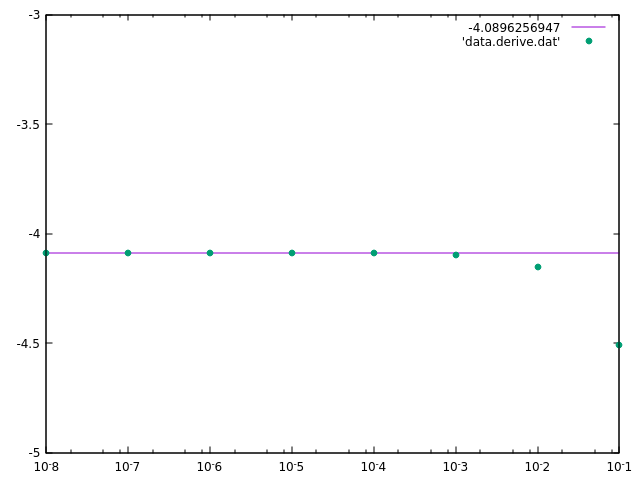
\includegraphics[scale=0.7]{derive.png}
	\caption*{{\scriptsize Gráfico 1 - $Eixo\ x\ em\ log,\ Derivada\ por\ \Delta t$}}
\end{figure}\\
\\
Considerando que uma boa aproximação considera um erro inferior a $1\%$, data venha que $f'_{aprox.}(3)= f'(3) \pm 1\% \text{de} f'(3)  = -4.0896 \pm 0.0409$, o que é obtido para pontos com valor de seu erro inferior a este.\\
\section{Solução Numérica de Equações Diferenciais}
Calculando a integral de $df/dt = F(f,t)$, com $F(f,t)$ dado por
\begin{equation}
F(f,t) = f + e^{\frac{t}{2}}\left[5\cos(5t)-\frac{1}{2}\sin(5t)\right],
\end{equation}
utilizando a condição de contorno $f(0) = 1$, usando o Método de Euler onde temos que os passos de discretização, $\Delta t$, são $0.1,\ 0.05,\ 0.01,\ 0.005,$ e $0.001$ e comparando com a solução exata, $f_{exata}(t)$ nos pontos $1,\ 2,\ 3,\ 4,$ e $5$, onde $f_{exata}(t)$ e o Método de Euler são dados por, respectivamente,
\begin{equation}
f(t) = e^t + e^{\frac{t}{2}}\sin(5t),
\end{equation}
\begin{equation}
f_{n+1} = f_n + F(f_n,t_n)\Delta t,
\end{equation}
obtemos a seguinte tabela:
\begin{center}
Método de Euler (Tabela 2)\\
\begin{tabular}{c c c c c c} 
\hline
$t$ & $\Delta t$ & $f_{exata}(t)$ & $f_{n}(t)$ & $\vert\vert f_{exata}(t)-f_{n}(t)\vert\vert$ & $erro\ \%$\\
\hline
$	1.00	$	&	$	0.1	$	&	$	1.1372829798	$	&	$	1.6220709091	$	&	$	0.4847879293	$	&	$	29.89	$	\\
$	1.00	$	&	$	0.05	$	&	$	1.1372829798	$	&	$	1.3881811114	$	&	$	0.2508981316	$	&	$	18.07	$	\\
$	1.00	$	&	$	0.01	$	&	$	1.1372829798	$	&	$	1.1890129837	$	&	$	0.0517300039	$	&	$	4.35	$	\\
$	1.00	$	&	$	0.005	$	&	$	1.1372829798	$	&	$	1.1632513042	$	&	$	0.0259683244	$	&	$	2.23	$	\\
$	1.00	$	&	$	0.001	$	&	$	1.1372829798	$	&	$	1.1424933910	$	&	$	0.0052104111	$	&	$	0.46	$	\\
\\																							
$	2.00	$	&	$	0.1	$	&	$	5.9102533989	$	&	$	7.3802034298	$	&	$	1.4699500309	$	&	$	19.92	$	\\
$	2.00	$	&	$	0.05	$	&	$	5.9102533989	$	&	$	6.6967203456	$	&	$	0.7864669467	$	&	$	11.74	$	\\
$	2.00	$	&	$	0.01	$	&	$	5.9102533989	$	&	$	6.0769482343	$	&	$	0.1666948354	$	&	$	2.74	$	\\
$	2.00	$	&	$	0.005	$	&	$	5.9102533989	$	&	$	5.9942290829	$	&	$	0.0839756840	$	&	$	1.40	$	\\
$	2.00	$	&	$	0.001	$	&	$	5.9102533989	$	&	$	5.9271504404	$	&	$	0.0168970415	$	&	$	0.29	$	\\
\\																							
$	3.00	$	&	$	0.1	$	&	$	22.9999248290	$	&	$	24.7514918596	$	&	$	1.7515670306	$	&	$	7.08	$	\\
$	3.00	$	&	$	0.05	$	&	$	22.9999248290	$	&	$	24.0260078092	$	&	$	1.0260829802	$	&	$	4.27	$	\\
$	3.00	$	&	$	0.01	$	&	$	22.9999248290	$	&	$	23.2333484030	$	&	$	0.2334235740	$	&	$	1.00	$	\\
$	3.00	$	&	$	0.005	$	&	$	22.9999248290	$	&	$	23.1185491605	$	&	$	0.1186243315	$	&	$	0.51	$	\\
$	3.00	$	&	$	0.001	$	&	$	22.9999248290	$	&	$	23.0239608597	$	&	$	0.0240360307	$	&	$	0.10	$	\\
\\																							
$	4.00	$	&	$	0.1	$	&	$	61.3439537060	$	&	$	60.8205391378	$	&	$	0.5234145683	$	&	$	0.86	$	\\
$	4.00	$	&	$	0.05	$	&	$	61.3439537060	$	&	$	61.4098321184	$	&	$	0.0658784124	$	&	$	0.11	$	\\
$	4.00	$	&	$	0.01	$	&	$	61.3439537060	$	&	$	61.4221962495	$	&	$	0.0782425435	$	&	$	0.13	$	\\
$	4.00	$	&	$	0.005	$	&	$	61.3439537060	$	&	$	61.3876097566	$	&	$	0.0436560506	$	&	$	0.07	$	\\
$	4.00	$	&	$	0.001	$	&	$	61.3439537060	$	&	$	61.3534268549	$	&	$	0.0094731489	$	&	$	0.02	$	\\
\\																							
$	5.00	$	&	$	0.1	$	&	$	146.8007847063	$	&	$	139.3455062442	$	&	$	7.4552784622	$	&	$	5.35	$	\\
$	5.00	$	&	$	0.05	$	&	$	146.8007847063	$	&	$	143.7414355185	$	&	$	3.0593491878	$	&	$	2.13	$	\\
$	5.00	$	&	$	0.01	$	&	$	146.8007847063	$	&	$	146.3333355417	$	&	$	0.4674491646	$	&	$	0.32	$	\\
$	5.00	$	&	$	0.005	$	&	$	146.8007847063	$	&	$	146.5775119429	$	&	$	0.2232727634	$	&	$	0.15	$	\\
$	5.00	$	&	$	0.001	$	&	$	146.8007847063	$	&	$	146.7578530251	$	&	$	0.0429316812	$	&	$	0.03	$	\\


\hline




\end{tabular}
\end{center}
Plotando o gráfico da solução pelo Método de Euler por tempo, com o valor fixo de $\Delta t = 0.05$ contra a solução exata da função, temos:\\
\begin{figure}[h!]
	\centering
	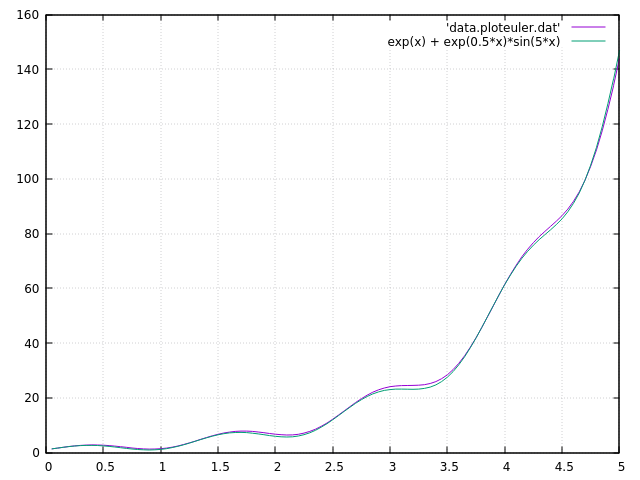
\includegraphics[scale=0.7]{euler.png}
	\caption*{{\scriptsize Gráfico 2 - $f_{n}(t)\ no\ eixo\ y\ e\ t\ no\ eixo\ x$ }}
\end{figure}\\
\\
\newpage
Com o bojetivo de se aprofundar no estudo das soluções numéricas de Equações Diferenciais, exploramos também outro método a fim de comparar os resultados obtidos a posterio. sendo utilizado o Método de Runge-Kutta de 2ª e 4ª ordem, com os mesmos passos de discretização. Temos que o Runge-Kutta de segunda ordem é dado por:
\begin{equation}
\begin{aligned}
k_1 &= F(f_n,t_n)\\
k_2 &= F(f_n+k_1\Delta t,t_n+\Delta t)\\
f_{n+1} &= f_n + \frac{\Delta t}{2}(k_1+k_2),
\end{aligned}
\end{equation}
Temos também que o Runge-Kutta de quarta ordem é dado por
\begin{equation}
\begin{aligned}
k_1 &= F(f_n,t_n)\\
k_2 &= F\left(f_n+\frac{1}{2}k_1\Delta t,t_n+\frac{1}{2}\Delta t\right)\\
k_3 &= F\left(f_n+\frac{1}{2}k_2\Delta t,t_n+\frac{1}{2}\Delta t\right)\\
k_4 &=  F(f_n+k_3\Delta t,t_n+\Delta t)\\
f_{n+1} &= f_n + \frac{\Delta t}{6}(k_1+2[k_2+k_3]+k_4).
\end{aligned}
\end{equation}
Fazendo a mesma comparação feita para o método de Euler, obtemos as seguintes tabelas
\begin{center}
\newpage
Método Runge-Kutta de 2ª Ordem (Tabela 3)\\
\begin{tabular}{c c c c c c} 
\hline
$t$ & $\Delta t$ & $f_{n}(t)$ & $f_{exata}(t)$ & $\vert\vert f_{exata}(t)-f_{n}(t)\vert\vert$ & $erro\ \%$\\
\hline 
$	1.00	$&$	0.1		$&$	1.1768098396	$&$	1.1372829798	$&$	0.0395268598	$&$	3.35881	$\\
$	1.00	$&$	0.05	$&$	1.1472865657	$&$	1.1372829798	$&$	0.0100035858	$&$	0.87193	$\\
$	1.00	$&$	0.01	$&$	1.1376878241	$&$	1.1372829798	$&$	0.0004048443	$&$	0.03558	$\\
$	1.00	$&$	0.005	$&$	1.1373843499	$&$	1.1372829798	$&$	0.0001013701	$&$	0.00891	$\\
$	1.00	$&$	0.001	$&$	1.1372870398	$&$	1.1372829798	$&$	0.0000040600	$&$	0.00036	$\\
\\												
$	2.00	$&$	0.1	    $&$	5.9533413846	$&$	5.9102533989	$&$	0.0430879857	$&$	0.72376	$\\
$	2.00	$&$	0.05	$&$	5.9214227128	$&$	5.9102533989	$&$	0.0111693139	$&$	0.18863	$\\
$	2.00	$&$	0.01	$&$	5.9107154192	$&$	5.9102533989	$&$	0.0004620203	$&$	0.00782	$\\
$	2.00	$&$	0.005	$&$	5.9103694198	$&$	5.9102533989	$&$	0.0001160209	$&$	0.00196	$\\
$	2.00	$&$	0.001	$&$	5.9102580565	$&$	5.9102533989	$&$	0.0000046576	$&$	0.00008	$\\
\\												
$	3.00	$&$	0.1		$&$	22.9176027358	$&$	22.9999248290	$&$	0.0823220932	$&$	0.35921	$\\
$	3.00	$&$	0.05	$&$	22.9798526734	$&$	22.9999248290	$&$	0.0200721556	$&$	0.08735	$\\
$	3.00	$&$	0.01	$&$	22.9991428988	$&$	22.9999248290	$&$	0.0007819301	$&$	0.00340	$\\
$	3.00	$&$	0.005	$&$	22.9997300753	$&$	22.9999248290	$&$	0.0001947537	$&$	0.00085	$\\
$	3.00	$&$	0.001	$&$	22.9999170626	$&$	22.9999248290	$&$	0.0000077663	$&$	0.00003	$\\
\\											
$	4.00	$&$	0.1		$&$	61.0222431740	$&$	61.3439537060	$&$	0.3217105320	$&$	0.52720	$\\
$	4.00	$&$	0.05	$&$	61.2633480374	$&$	61.3439537060	$&$	0.0806056686	$&$	0.13157	$\\
$	4.00	$&$	0.01	$&$	61.3407329736	$&$	61.3439537060	$&$	0.0032207325	$&$	0.00525	$\\
$	4.00	$&$	0.005	$&$	61.3431487767	$&$	61.3439537060	$&$	0.0008049294	$&$	0.00131	$\\
$	4.00	$&$	0.001	$&$	61.3439215179	$&$	61.3439537060	$&$	0.0000321881	$&$	0.00005	$\\
\\										
$	5.00	$&$	0.1		$&$	146.1425495890	$&$	146.8007847063	$&$	0.6582351173	$&$	0.45041	$\\
$	5.00	$&$	0.05	$&$	146.6334717248	$&$	146.8007847063	$&$	0.1673129815	$&$	0.11410	$\\
$	5.00	$&$	0.01	$&$	146.7940314375	$&$	146.8007847063	$&$	0.0067532688	$&$	0.00460	$\\
$	5.00	$&$	0.005	$&$	146.7990949190	$&$	146.8007847063	$&$	0.0016897873	$&$	0.00115	$\\
$	5.00	$&$	0.001	$&$	146.8007170705	$&$	146.8007847063	$&$	0.0000676358	$&$	0.00005	$\\
\hline
\end{tabular}
\end{center}
\newpage
\begin{center}
Método Runge-Kutta de 4ª Ordem (Tabela 4)\\
\begin{tabular}{c c c c c c} 
\hline
$t$ & $\Delta t$ & $f_{n}(t)$ & $f_{exata}(t)$ & $\vert\vert f_{exata}(t)-f_{n}(t)\vert\vert$ & $erro\ \%$\\
\hline 
$	1.00	$&$	0.1	$&$	1.13723777023248	$&$	1.13728297983124	$&$	0.00004520959876	$&$	0.00397538667300	$	\\
$	1.00	$&$	0.05	$&$	1.13728018266218	$&$	1.13728297983124	$&$	0.00000279716906	$&$	0.00024595250131	$	\\
$	1.00	$&$	0.01	$&$	1.13728297537613	$&$	1.13728297983124	$&$	0.00000000445510	$&$	0.00000039173220	$	\\
$	1.00	$&$	0.05	$&$	1.13728297955289	$&$	1.13728297983124	$&$	0.00000000027835	$&$	0.00000002447492	$	\\
$	1.00	$&$	0.01	$&$	1.13728297983079	$&$	1.13728297983124	$&$	0.00000000000044	$&$	0.00000000003903	$	\\
\\													
$	2.00	$&$	0.1	$&$	5.91015802851975	$&$	5.91025339890197	$&$	0.00009537038222	$&$	0.00161366890294	$	\\
$	2.00	$&$	0.05	$&$	5.91024756423233	$&$	5.91025339890197	$&$	0.00000583466964	$&$	0.00009872123935	$	\\
$	2.00	$&$	0.01	$&$	5.91025338969221	$&$	5.91025339890197	$&$	0.00000000920977	$&$	0.00000015582691	$	\\
$	2.00	$&$	0.05	$&$	5.91025339832753	$&$	5.91025339890197	$&$	0.00000000057445	$&$	0.00000000971952	$	\\
$	2.00	$&$	0.01	$&$	5.91025339890277	$&$	5.91025339890197	$&$	0.00000000000079	$&$	0.00000000001340	$	\\
\\													
$	3.00	$&$	0.1	$&$	22.99979845355124	$&$	22.99992482899356	$&$	0.00012637544232	$&$	0.00054946325977	$	\\
$	3.00	$&$	0.05	$&$	22.99991719938262	$&$	22.99992482899356	$&$	0.00000762961094	$&$	0.00003317234092	$	\\
$	3.00	$&$	0.01	$&$	22.99992481708318	$&$	22.99992482899356	$&$	0.00000001191038	$&$	0.00000005178445	$	\\
$	3.00	$&$	0.05	$&$	22.99992482825224	$&$	22.99992482899356	$&$	0.00000000074133	$&$	0.00000000322317	$	\\
$	3.00	$&$	0.01	$&$	22.99992482899752	$&$	22.99992482899356	$&$	0.00000000000396	$&$	0.00000000001722	$	\\
\\													
$	4.00	$&$	0.1	$&$	61.34361678880934	$&$	61.34395370602299	$&$	0.00033691721364	$&$	0.00054922945741	$	\\
$	4.00	$&$	0.05	$&$	61.34393306452798	$&$	61.34395370602299	$&$	0.00002064149501	$&$	0.00003364879618	$	\\
$	4.00	$&$	0.01	$&$	61.34395367341735	$&$	61.34395370602299	$&$	0.00000003260563	$&$	0.00000005315216	$	\\
$	4.00	$&$	0.05	$&$	61.34395370398758	$&$	61.34395370602299	$&$	0.00000000203541	$&$	0.00000000331802	$	\\
$	4.00	$&$	0.01	$&$	61.34395370601806	$&$	61.34395370602299	$&$	0.00000000000492	$&$	0.00000000000803	$	\\
\\													
$	5.00	$&$	0.1	$&$	146.79939737175198	$&$	146.80078470632193	$&$	0.00138733456996	$&$	0.00094505467651	$	\\
$	5.00	$&$	0.05	$&$	146.80069872436974	$&$	146.80078470632193	$&$	0.00008598195220	$&$	0.00005857053334	$	\\
$	5.00	$&$	0.01	$&$	146.80078456924392	$&$	146.80078470632193	$&$	0.00000013707802	$&$	0.00000009337690	$	\\
$	5.00	$&$	0.05	$&$	146.80078469775324	$&$	146.80078470632193	$&$	0.00000000856869	$&$	0.00000000583695	$	\\
$	5.00	$&$	0.01	$&$	146.80078470632725	$&$	146.80078470632193	$&$	0.00000000000531	$&$	0.00000000000362	$	\\
\hline

\end{tabular}
\end{center}
As tabelas são densas, dado o volume de dados analisado no problema, contudo é possível ver o quanto este método parece promissor em comparação com o Método de Euler.\\
%\footnote{Os valores da tabelas 2,3 e 4 foram ``arredondados'' para que fosse possível coloca-los em conjunto na tabela.}
\\
Novamente, fazendo o gráfico da solução pelo Método de Runge-Kutta por tempo, em 2ª e posteriormente o fazemos para 4ª ordem, com $\Delta t = 0.05$ em ambos, confrontando a solução exata, temos:
\newpage
\begin{figure}[h!]
	\centering
	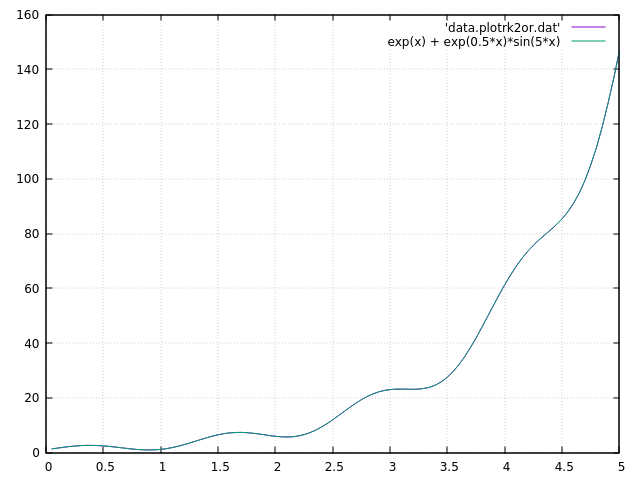
\includegraphics[scale=0.7]{rk2or.png}
	\caption*{{\scriptsize Gráfico 3}}
\end{figure}
Gráficamente é difícil enxergar discrepâncias entre as curvas, dando a impressão de que as mesmas são uma só. Nas tabélas 3 e 4 se observa um erro pequeno, da ordem de $10^{-4}$, é de se esperar que ao comparar graficamente os valores  em $t$ tivesse uma certa sobreposição devido a precisão do pacote gráfico.
\begin{figure}[h!]
	\centering
	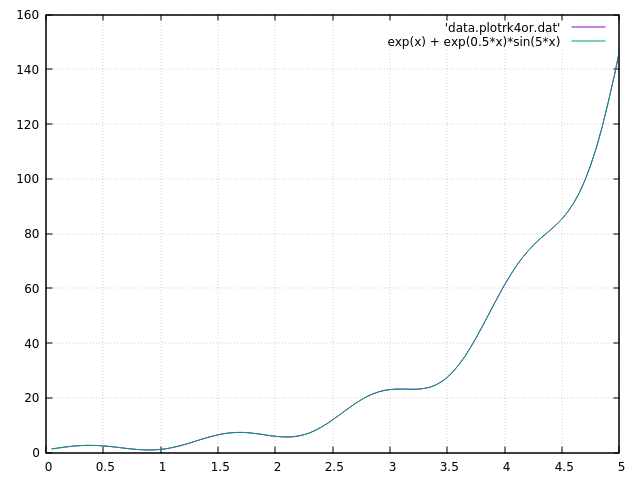
\includegraphics[scale=0.7]{rk4or.png}
	\caption*{{\scriptsize Gráfico 4}}
\end{figure}
Em suma, podemos verificar que para valores maiors de $\Delta t$ o Método de Euler pode fornecer bons resultados, contudo o Método de Ruge-Kutta de 4ª Ordem pode fornecer bons pontos com menos loopings, sendo mais apropriado para grandes volumes de dados que precisem seer tratados em um tempo curto.
\end{document}